% Name: Perceptron
% Description: Inputs, weights, a sum, and an activation: one artificial neuron.
% Tags: perceptron, neuron, activation

\usetikzlibrary{arrows.meta, positioning}

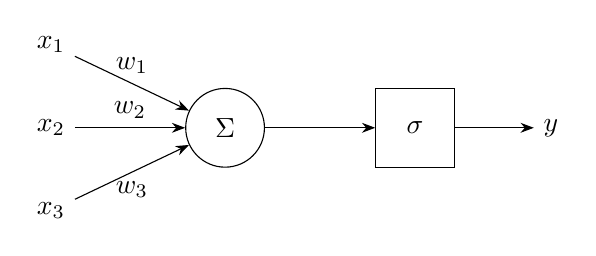
\begin{tikzpicture}[
  node distance=6mm and 14mm,
  every edge/.style={draw, -{Stealth}},
]
  \node[circle, draw, minimum size=10mm] (sum) {$\Sigma$};
  \node[left=of sum] (x2) {$x_2$};
  \node[above=of x2] (x1) {$x_1$};
  \node[below=of x2] (x3) {$x_3$};
  \node[draw, right=of sum, minimum size=10mm] (act) {$\sigma$};
  \node[right=10mm of act] (y) {$y$};

  \path (x1) edge node[above] {$w_1$} (sum)
        (x2) edge node[above] {$w_2$} (sum)
        (x3) edge node[below] {$w_3$} (sum)
        (sum) edge (act)
        (act) edge (y);
\end{tikzpicture}
